{\textbf{1. 外部排序的基本概念}}

{内排序就是可以在内存中完成的排序(如快速排序、堆排序、归并排序等)。区别于内排序,外部排序指的是大文件的排序,即待排序的记录存储在外存储器上,待排序的文件无法一次装入内存。{外部排序最常用的算法是多路归并排序},分为两步:}

{① 将文件中的数据分段输入内存,用内排的方法进行排序,然后写回到外存;}

{② 对这些有序段,采用归并方法,在外存上形成整个文件的单一归并段。}{}

{\textbf{2. 最佳归并树}}

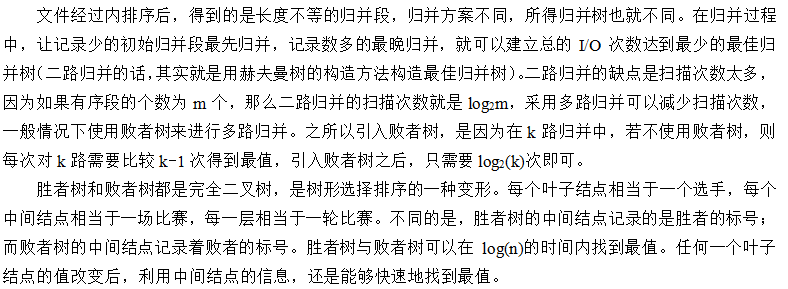
\includegraphics[width=3.70833in,height=1.36458in]{png-jpeg-pics/7C0D015232CDC8CB5F63EF614F3C2D0A.png}

{\textbf{3. 胜者树}}

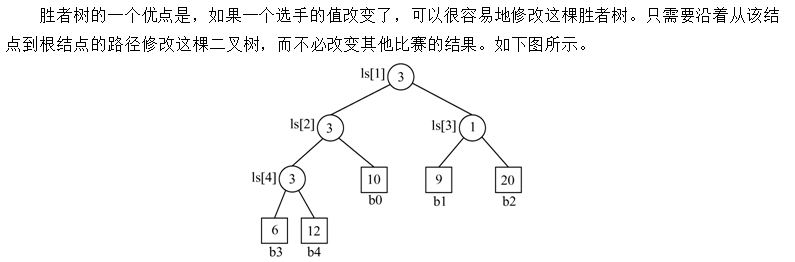
\includegraphics[width=3.70833in,height=1.21875in]{png-jpeg-pics/144878B1DFDF623E5FD212A310E768B5.png}

{\textbf{4. 败者树}}

{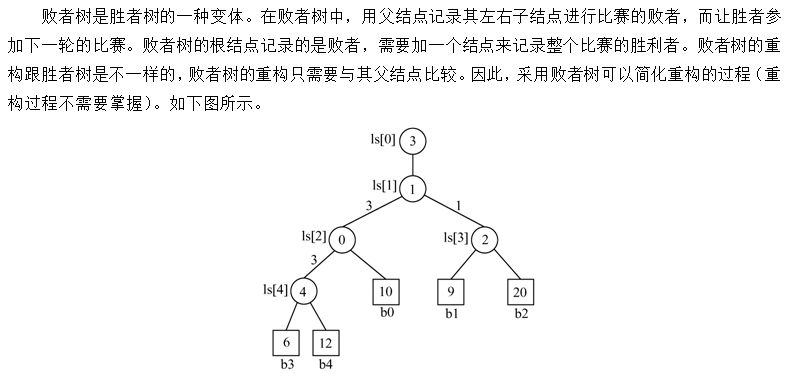
\includegraphics[width=3.70833in,height=1.75000in]{png-jpeg-pics/0D1188BB7CAF6C367D56C201AB36812E.png}}
